\part{Rastreabilidade dos requisitos}
\chapter[Rastreabilidade dos requisitos]{Rastreabilidade dos requisitos}

A gerência dos requistos está associada às atividades que acompanham o desenvolvimento do requisito em seus vários níveis de abstração. Dessa forma, é possível identificar sua importância caso se leve em conta o fato de que a mudança de um requisito, independentemente do seu nível de abstração, pode acarretar na mudança de vários artefatos, até mesmo aterfatos de desenho, e caso não se saiba de onde um requisito veio e para onde ele vai, essa mudança, mesmo que simples, pode gerar grandes falhas no projeto \cite{sayao2006rastreabilidade}.

Tendo essas assertivas em mente, utilizou-se da ferramenta online Innoslate para auxiliar a gerência de requisitos do projeto, garantindo assim uma menor chance de falhas na documentação.

A rastreabilidade foi realizada da seguinte forma: a partir do problema identificado no contexto em questão, foram apontadas as necessidades dos envolvidos e dos usuários. Uma vez apontadas as necessidades, foram levantados requisitos funcionais e não funcionais referentes a essas necessidades. Feito isso, foram definidos os casos de uso que atendem aos requisitos levantados. Todo esse processo foi realizado com o auxílio das técnicas de elicitação detalhadas em \ref{sec:tec}.

A figura \ref{fig:rastnec} representa a parte do processo de rastreabilidade comentado, que diz respeito à relação entre necessidades dos envolvidos e dos usuário com os requisitos funcionais e não-funcionais do projeto. Já a figura \ref{fig:rastuc} diz respeito a última parte do processo da gerência dos requisitos, a qual está relacionada com a conexão entre os requisitos do projeto e os casos de uso que atendem esses requisitos. Por fim, a figura \ref{fig:diag} representa o diagrama de rastreabilidade do projeto, que é todo esse processo de gerência dos requisitos resumido em uma imagem.

Os identificadores referentes às necessidades podem ser encontrados no documento de visão em \ref{doc:visao} e os identificadores referentes aos requisitos no documento de arquitetura em \ref{doc:arq}. P01 diz respeito ao problema que se quer resolver, detalhado em \ref{doc:cont} e \ref{doc:visao}.

\begin{figure}[h!]
	\centering
	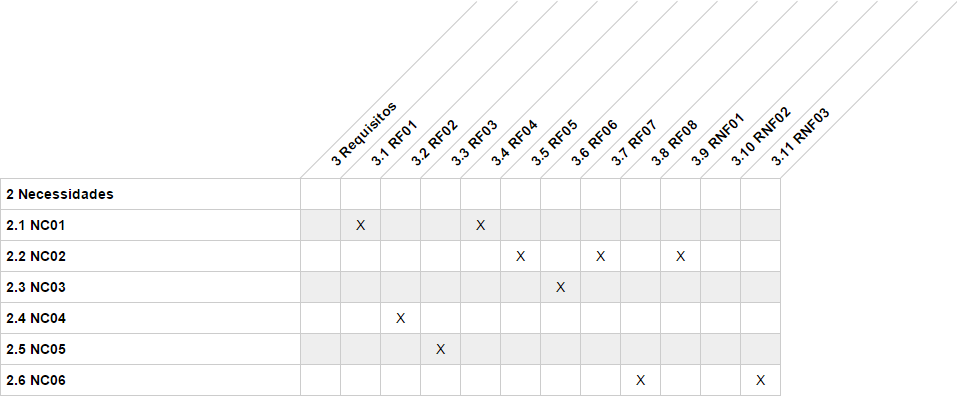
\includegraphics[width=\textwidth]{figuras/rastnec.png}
	\caption{Relação entre as necessidades dos envolvidos/usuários e os requisitos do projeto}
	\label{fig:rastnec}
\end{figure}

\begin{figure}[h!]
	\centering
	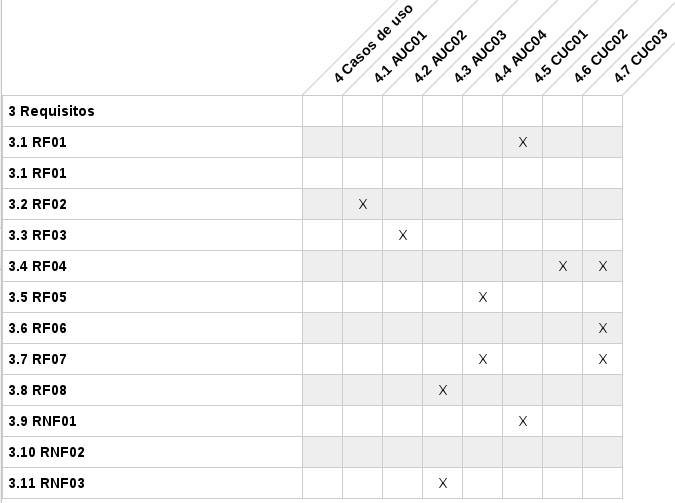
\includegraphics[width=\textwidth]{figuras/rastuc.png}
	\caption{Relação entre os requisitos e os casos de uso do projeto}
	\label{fig:rastuc}
\end{figure}

\begin{figure}[h!]
	\centering
	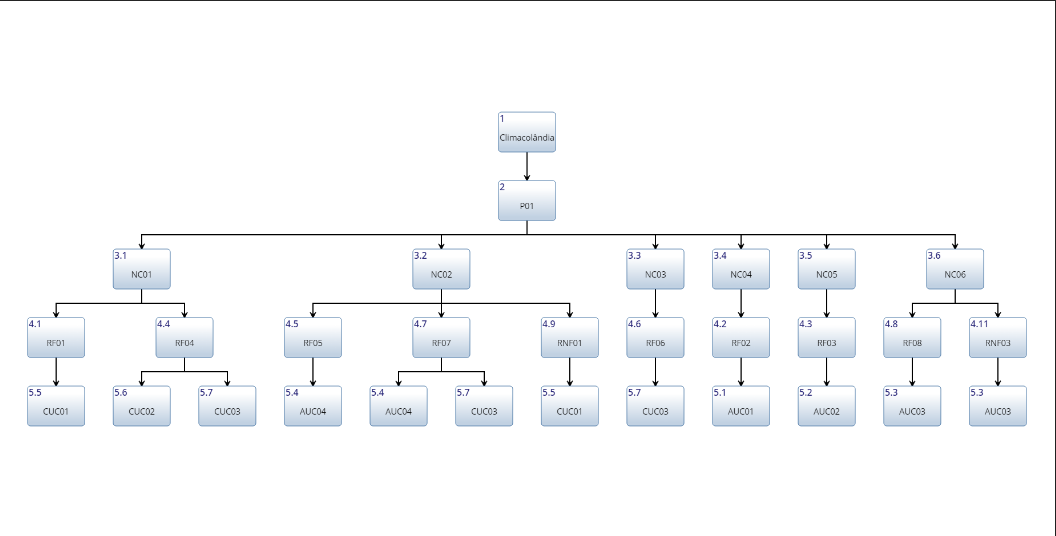
\includegraphics[width=\textwidth]{figuras/diag.png}
	\caption{Diagrama de rastreabilidade do projeto}
	\label{fig:diag}
\end{figure}